\documentclass[conference,10pt]{IEEEtran}
\IEEEoverridecommandlockouts

\usepackage[utf8]{inputenc}
\usepackage[T1]{fontenc}
\usepackage{mathptmx}
\usepackage{amsmath,amssymb}
\usepackage{booktabs}
\usepackage{tabularx}
\usepackage{array}
\usepackage{multirow}
\usepackage{graphicx}
\usepackage{xcolor}
\usepackage{listings}
\usepackage{caption}
\usepackage{subcaption}
\usepackage{enumitem}
\usepackage{hyperref}

\hypersetup{
    colorlinks=true,
    linkcolor=blue!60!black,
    urlcolor=blue!60!black,
    citecolor=blue!60!black,
    pdftitle={RTL-to-GDSII Design and Implementation of a 4-Bit Registered Array Multiplier in SkyWater 130 nm CMOS},
    pdfauthor={Manikya Pant (2023112024), Aryan Agrawal (2023102050)}
}

\setlength{\emergencystretch}{2em}
\renewcommand{\dbltopfraction}{0.92}
\renewcommand{\topfraction}{0.92}
\renewcommand{\bottomfraction}{0.85}
\renewcommand{\textfraction}{0.07}
\renewcommand{\floatpagefraction}{0.85}
\renewcommand{\dblfloatpagefraction}{0.85}
\setcounter{topnumber}{4}
\setcounter{dbltopnumber}{4}
\setcounter{totalnumber}{6}

\setlist[itemize]{leftmargin=1.2em,itemsep=1pt,topsep=2pt,parsep=0pt}
\setlist[enumerate]{leftmargin=1.4em,itemsep=1pt,topsep=2pt,parsep=0pt}

\captionsetup{font=footnotesize,labelfont=bf,skip=3pt}

\definecolor{codebg}{RGB}{247,248,250}
\definecolor{codeframe}{RGB}{210,215,222}

\lstset{
    basicstyle=\ttfamily\scriptsize,
    backgroundcolor=\color{codebg},
    frame=single,
    rulecolor=\color{codeframe},
    framesep=2.5pt,
    xleftmargin=3pt,
    xrightmargin=3pt,
    aboveskip=4pt,
    belowskip=4pt,
    breaklines=true,
    columns=fullflexible,
    keepspaces=true,
    showstringspaces=false
}

\title{RTL-to-GDSII Design and Implementation of a\\4-Bit Registered Array Multiplier in SkyWater 130\,nm CMOS}

\author{
\IEEEauthorblockN{Manikya Pant}
\IEEEauthorblockA{\textit{Roll Number: 2023112024}\\
Digital VLSI Design, IIIT Hyderabad\\
manikya.pant@research.iiit.ac.in\\
\textbf{GitHub}: \url{https://github.com/ManikyaPant/DVD_assignment}}
\and
\IEEEauthorblockN{Aryan Agrawal}
\IEEEauthorblockA{\textit{Roll Number: 2023102050}\\
Digital VLSI Design, IIIT Hyderabad\\
aryan.agrawal@students.iiit.ac.in\\
\textbf{GitHub}: \url{https://github.com/ManikyaPant/DVD_assignment}}
\thanks{GitHub Repository: \url{https://github.com/ManikyaPant/DVD_assignment}}
}

\begin{document}

\maketitle

\begin{abstract}
This report presents the complete end-to-end open-source RTL-to-GDSII implementation of a 4-bit unsigned registered array multiplier (\texttt{mult\_array}) in the SkyWater 130\,nm CMOS process (\texttt{sky130A}, standard-cell library \texttt{sky130\_fd\_sc\_hd}). The architecture comprises 16 two-input partial-product AND gates, 12 full adders arranged in three 4-bit ripple-carry rows, 8 input flip-flops, and 8 output flip-flops, providing a 2-clock-cycle latency and 1-result/cycle throughput. Exhaustive self-checking verification in Icarus Verilog across all 256 input vectors passes with 0 errors in both behavioral and gate-level simulation, while an error-injection test (\texttt{sum = a \^{} b}) catches 95 errors. Yosys synthesis maps the design to 67 cells ($746.966\,\mu\text{m}^2$, $53.60\%$ flip-flop area). Pre-layout OpenSTA analysis yields $T_{\min} = 2.604\text{ ns}$ ($F_{\max} = 384.02\text{ MHz}$) along an 8-cell combinational critical path from \texttt{b\_reg[0]} to \texttt{p[6]}. Physical implementation in LibreLane/OpenROAD on a $150\,\mu\text{m} \times 150\,\mu\text{m}$ die converges in 8 clock-period iterations at $T_{\text{clk}} = 7.0\text{ ns}$ ($F_{\max} = 153.01\text{ MHz}$ worst-case \texttt{max\_ss\_100C\_1v60}, $316.34\text{ MHz}$ nominal \texttt{nom\_tt\_025C\_1v80}) with 0 DRC and 0 LVS violations.
\end{abstract}

\begin{IEEEkeywords}
Array multiplier, RTL-to-GDSII, SkyWater SKY130, Yosys, OpenSTA, LibreLane, OpenROAD, DRC, LVS.
\end{IEEEkeywords}

% ==================== I. INTRODUCTION ====================
\section{Introduction}
Binary multiplication is a fundamental arithmetic operation in digital signal processors, general-purpose microprocessors, and hardware accelerators. This work implements and characterizes a 4-bit $\times$ 4-bit unsigned registered array multiplier (\texttt{mult\_array}) through a complete open-source RTL-to-GDSII flow inside the IIC-OSIC-TOOLS environment targeting the SkyWater 130\,nm high-density standard-cell library (\texttt{sky130\_fd\_sc\_hd}, nominal corner \texttt{tt\_025C\_1v80} at $V_{\text{DD}} = 1.80\text{ V}, T = 25\,^\circ\text{C}$). All design files, scripts, and reports are available in the project GitHub repository at \url{https://github.com/ManikyaPant/DVD_assignment}.

Given two 4-bit unsigned operands $A = a_3a_2a_1a_0 \in [0, 15]$ and $B = b_3b_2b_1b_0 \in [0, 15]$, the multiplier computes the 8-bit unsigned product $P = p_7p_6p_5p_4p_3p_2p_1p_0 = A \times B \in [0, 225]$ via binary shift-and-add:
\begin{equation}
    P = \sum_{i=0}^{3} \left( A \cdot b_i \right) 2^i = \sum_{i=0}^{3} \sum_{j=0}^{3} (a_j \wedge b_i)\,2^{i+j}
\end{equation}
The combinational core uses \textbf{16 two-input AND gates} to form four 4-bit partial products $\text{pp}_i[j] = a_j \wedge b_i$ and \textbf{12 1-bit full adders} arranged in three 4-bit ripple-carry adder rows (\texttt{row1}, \texttt{row2}, \texttt{row3}). Registering the two 4-bit inputs (\texttt{a\_reg[3:0]}, \texttt{b\_reg[3:0]}) and the 8-bit product (\texttt{p[7:0]}) on the rising edge of \texttt{clk} with active-low asynchronous reset (\texttt{rst\_n}) uses \textbf{16 flip-flops}, resulting in a \textbf{2-clock-cycle latency} and a \textbf{throughput of 1 result per clock cycle}.

% ==================== II. DESIGN AND VERIFICATION (PART A) ====================
\section{Design and Verification (Part A)}

\subsection{RTL Architecture and Exact Connections}
The synthesizable RTL is written in two Verilog modules without using the \texttt{*} operator:
\begin{itemize}
    \item \texttt{rtl/full\_adder.v}: A 1-bit combinational full adder with inputs \texttt{a}, \texttt{b}, \texttt{cin} and outputs \texttt{sum}, \texttt{cout} implemented with \texttt{assign} statements:
    \texttt{assign sum = a \^{} b \^{} cin;} and \texttt{assign cout = (a \& b) | (b \& cin) | (cin \& a);}.
    \item \texttt{rtl/mult\_array.v}: Registers \texttt{a[3:0]} and \texttt{b[3:0]} into \texttt{a\_reg[3:0]} and \texttt{b\_reg[3:0]} on \texttt{posedge clk} (or clears all registers to $0$ on \texttt{negedge rst\_n}). Sixteen AND gates form $\texttt{pp0} = \texttt{a\_reg \& \{4\{b\_reg[0]\}\}}$ through $\texttt{pp3}$. Row 0 produces $\texttt{p[0]} = \texttt{pp0[0]}$ and passes $\texttt{r0} = \texttt{\{1'b0, pp0[3:1]\}}$ to Row 1. Rows 1--3 instantiate 12 \texttt{full\_adder} modules via a \texttt{generate} loop (\texttt{adder\_columns[0..3].row1..3}) with $\texttt{c1[0]} = \texttt{c2[0]} = \texttt{c3[0]} = \texttt{1'b0}$, passing $\texttt{r1} = \texttt{\{c1[4], s1[3:1]\}}$ and $\texttt{r2} = \texttt{\{c2[4], s2[3:1]\}}$ downward and registering $\texttt{product} = \texttt{\{c3[4], s3[3:1], s3[0], s2[0], s1[0], pp0[0]\}}$ into \texttt{p[7:0]}.
\end{itemize}
Fig.~\ref{fig:block_diagram} shows the complete structural block diagram of \texttt{mult\_array}.

\begin{figure}[!t]
    \centering
    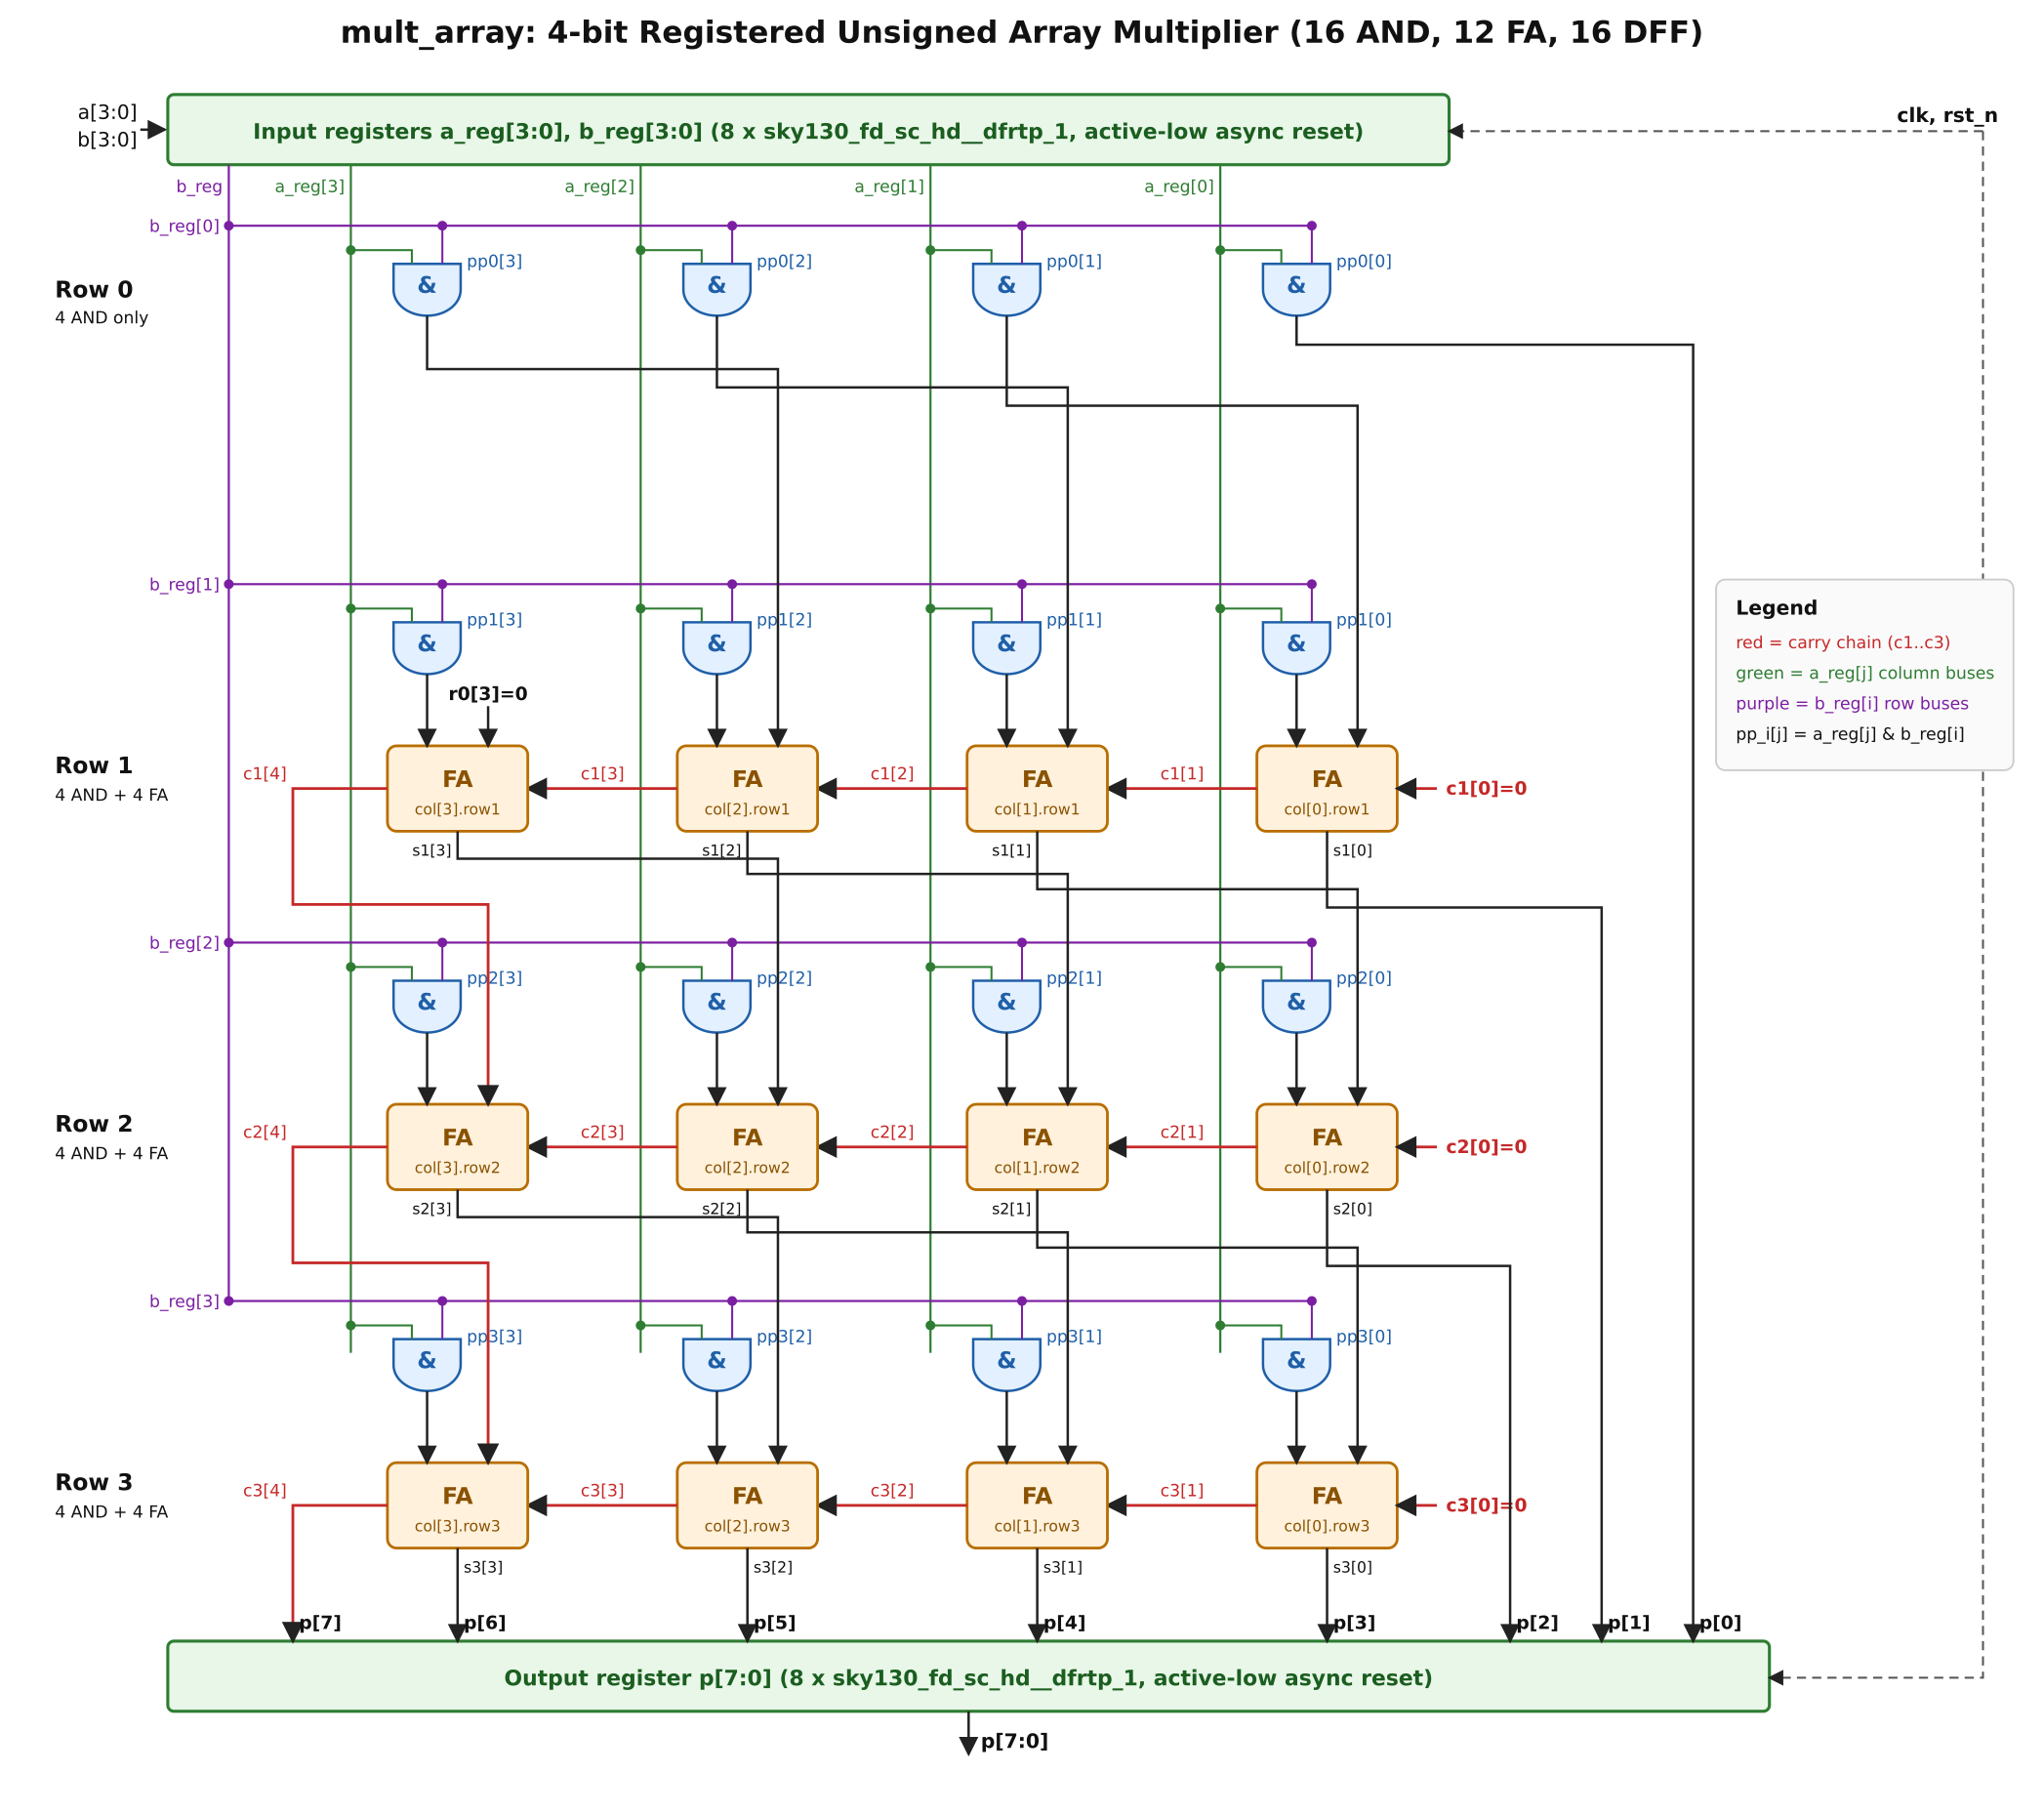
\includegraphics[width=0.96\columnwidth]{figures/partA_block_diagram.png}
    \caption{Structural block diagram of \texttt{mult\_array} showing the 8-bit input register bank (\texttt{a\_reg[3:0]}, \texttt{b\_reg[3:0]}), 16 partial-product AND gates (\texttt{pp0}--\texttt{pp3}), 12 full adders across three 4-bit ripple-carry rows (\texttt{row1}--\texttt{row3}), and the 8-bit output register (\texttt{p[7:0]}).}
    \label{fig:block_diagram}
\end{figure}

\subsection{Hand-Worked Example for Roll Number \texttt{2023112024} ($A = 9, B = 7$)}
Using Manikya Pant's roll number \texttt{2023112024}, the last digit is $d = 4$, giving $A = 4 + 5 = 9 = 1001_2$ (\texttt{4'b1001}) and $B = 7 = 0111_2$ (\texttt{4'b0111}), with expected product $P = 9 \times 7 = 63 = 00111111_2$ (\texttt{8'h3F}). The binary shift-and-add calculation and internal row-by-row hardware trace in \texttt{rtl/mult\_array.v} are shown below:

\begin{lstlisting}[title={\textbf{Hand-Worked Multiplication ($A = 9, B = 7 \rightarrow P = 63$)}}]
        1 0 0 1   A = 9 (roll 2023112024: last digit 4 + 5)
      x 0 1 1 1   B = 7
---------------
        1 0 0 1   pp0 = A AND b0 (b0 = 1) -> p[0]=1, r0=0100
      1 0 0 1     pp1 = A AND b1 (b1 = 1), shifted 1
    1 0 0 1       pp2 = A AND b2 (b2 = 1), shifted 2
  0 0 0 0         pp3 = A AND b3 (b3 = 0), shifted 3
---------------
0 0 1 1 1 1 1 1   P = 63 (0x3F = 32 + 16 + 8 + 4 + 2 + 1)

Row 0: pp0 = 4'b1001 -> p[0] = pp0[0] = 1; r0 = {0,pp0[3:1]} = 4'b0100
Row 1: pp1 (1001) + r0 (0100), c1[0]=0 -> s1=1101, c1[4:1]=0000
       -> p[1] = s1[0] = 1; passes r1 = {c1[4], s1[3:1]} = 4'b0110
Row 2: pp2 (1001) + r1 (0110), c2[0]=0 -> s2=1111, c2[4:1]=0000
       -> p[2] = s2[0] = 1; passes r2 = {c2[4], s2[3:1]} = 4'b0111
Row 3: pp3 (0000) + r2 (0111), c3[0]=0 -> s3=0111, c3[4:1]=0000
       -> p[3] = s3[0] = 1; p[7:4] = {c3[4], s3[3:1]} = 4'b0011
Final: product[7:0] = 8'b0011_1111 = 63 (0x3F)
\end{lstlisting}

\begin{figure}[!t]
    \centering
    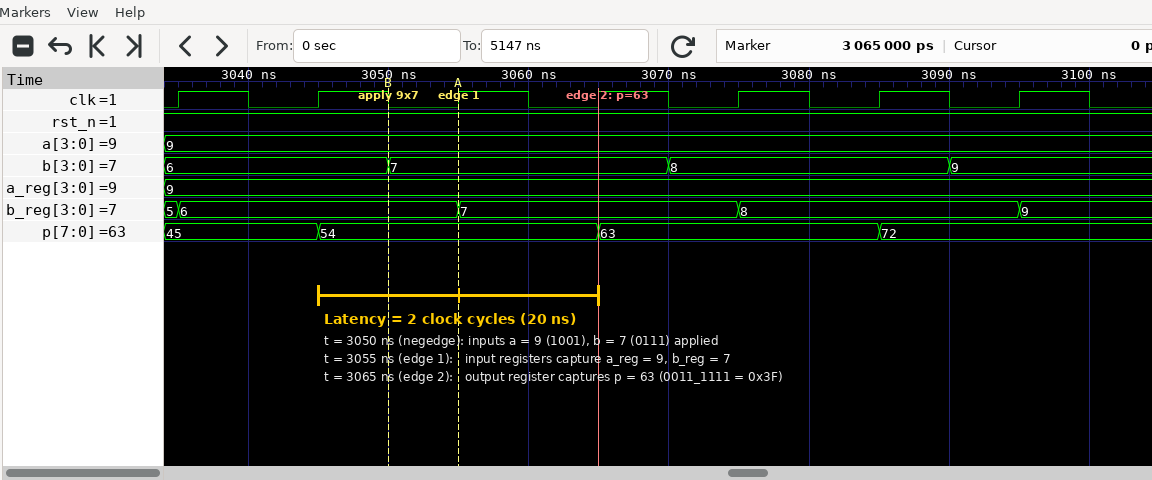
\includegraphics[width=0.98\columnwidth]{figures/partA_waveform.png}
    \caption{GTKWave waveform (\texttt{mult.vcd}) for $A = 9, B = 7 \rightarrow P = 63$ (\texttt{0x3F}) at $T_{\text{clk}} = 10.0\text{ ns}$: inputs applied at $t = 3050\text{ ns}$, captured into \texttt{a\_reg}/\texttt{b\_reg} at rising edge 1 ($t = 3055\text{ ns}$), and product $p = 63$ latched into \texttt{p[7:0]} at rising edge 2 ($t = 3065\text{ ns}$), showing the 2-clock-cycle ($20.0\text{ ns}$) latency.}
    \label{fig:waveform}
\end{figure}

% Queue Table II for top of Page 3
\begin{table*}[!t]
    \centering
    \caption{Complete 23-Cell-Type Breakdown of Synthesized \texttt{mult\_array} from \texttt{synth/mult\_array\_stat.rpt} (\texttt{sky130\_fd\_sc\_hd}).}
    \label{tab:partB_breakdown}
    \footnotesize
    \begin{tabularx}{\textwidth}{@{}X r r | X r r@{}}
        \toprule
        \textbf{Cell Type (\texttt{sky130\_fd\_sc\_hd\_\_*})} & \textbf{Count} & \textbf{Area ($\mu\text{m}^2$)} & \textbf{Cell Type (\texttt{sky130\_fd\_sc\_hd\_\_*})} & \textbf{Count} & \textbf{Area ($\mu\text{m}^2$)} \\
        \midrule
        \texttt{dfrtp\_1} (Pos-edge DFF w/ async active-low reset) & 16 & 400.384 & \texttt{a21boi\_0} (2-1 AND-OR-Invert w/ inverted B1\_N) & 1 & 7.507 \\
        \texttt{nand2\_1} (2-input NAND gate) & 12 & 45.043 & \texttt{a22oi\_1} (2-2 AND-OR-Invert gate) & 1 & 7.507 \\
        \texttt{xnor2\_1} (2-input XNOR gate) & 7 & 61.309 & \texttt{a32oi\_1} (3-2 AND-OR-Invert gate) & 1 & 8.758 \\
        \texttt{a21oi\_1} (2-1 AND-OR-Invert gate) & 4 & 20.019 & \texttt{and4\_1} (4-input AND gate) & 1 & 8.758 \\
        \texttt{and2\_0} (2-input AND gate) & 2 & 12.512 & \texttt{clkinv\_1} (Balanced clock inverter) & 1 & 3.754 \\
        \texttt{lpflow\_isobufsrc\_1} (Low-power isolation buffer) & 2 & 12.512 & \texttt{nand3\_1} (3-input NAND gate) & 1 & 5.005 \\
        \texttt{maj3\_1} (3-input majority carry gate) & 2 & 20.019 & \texttt{nor2\_1} (2-input NOR gate) & 1 & 3.754 \\
        \texttt{nand2b\_1} (2-input NAND w/ inverted input A\_N) & 2 & 12.512 & \texttt{o21ba\_1} (2-1 OR-AND w/ inverted input B1\_N) & 1 & 10.010 \\
        \texttt{nand4\_1} (4-input NAND gate) & 2 & 12.512 & \texttt{or3\_1} (3-input OR gate) & 1 & 6.256 \\
        \texttt{nor3\_1} (3-input NOR gate) & 2 & 10.010 & \texttt{xor2\_1} (2-input XOR gate) & 1 & 8.758 \\
        \texttt{o21a\_1} (2-1 OR-AND gate) & 2 & 15.014 & & & \\
        \texttt{o21ai\_0} (2-1 OR-AND-Invert gate) & 2 & 10.010 & & & \\
        \texttt{xnor3\_1} (3-input XNOR gate) & 2 & 45.043 & \textbf{Total (23 distinct standard-cell types)} & \textbf{67} & \textbf{746.966} \\
        \bottomrule
    \end{tabularx}
\end{table*}

\subsection{Exhaustive Verification, Passed Run, and Failed Injection}
The self-checking testbench (\texttt{tb/tb\_mult.v}) drives a $10\text{ ns}$ clock ($100\text{ MHz}$), holds \texttt{rst\_n = 0} for the first 2 rising clock edges, and applies all $256$ input combinations $(a, b) \in [0, 15]^2$ on \texttt{negedge clk}. For each combination, it waits 2 rising clock edges (2-cycle latency) plus \texttt{\#2}\,ns before comparing \texttt{p} against \texttt{expected = a\_value * b\_value}, and writes \texttt{mult.vcd} (Fig.~\ref{fig:waveform}).
\begin{itemize}
    \item \textbf{Passed Run (Task 4, \texttt{sum = a \^{} b \^{} cin})}: Compiling and running \texttt{iverilog -g2012 -o sim tb/tb\_mult.v rtl/full\_adder.v rtl/mult\_array.v \&\& vvp sim} checks all 256 vectors and prints \texttt{PASS: 256 vectors checked, 0 errors}.
    \item \textbf{Failed Error-Injection Run (Task 6, \texttt{sum = a \^{} b})}: Temporarily changing \texttt{sum} in \texttt{rtl/full\_adder.v} to \texttt{a \^{} b} (omitting \texttt{\^{} cin}) corrupts the sum output whenever any full adder receives $\texttt{cin} = 1$, causing \textbf{95 mismatches out of 256 vectors} and printing \texttt{FAIL: 256 vectors checked, 95 errors} (complete 95-mismatch log in Appendix~\ref{app:logs}). Restoring \texttt{sum = a \^{} b \^{} cin} restores \texttt{PASS}.
\end{itemize}

\begin{lstlisting}[title={\textbf{Part A Passed Run and Failed Error-Injection Summary Lines}}]
# Task 4: Passed RTL Run (unmodified rtl/full_adder.v)
VCD info: dumpfile mult.vcd opened for output.
PASS: 256 vectors checked, 0 errors
tb/tb_mult.v:75: $finish called at 5146000 (1ps)

# Task 6: Failed Error-Injection Run (sum = a ^ b in rtl/full_adder.v)
VCD info: dumpfile mult.vcd opened for output.
Mismatch: a=3 b=3 expected=9 got=5
Mismatch: a=3 b=6 expected=18 got=10
... [91 intermediate mismatches; full 95-error log in Appendix A] ...
Mismatch: a=15 b=15 expected=225 got=181
FAIL: 256 vectors checked, 95 errors
tb/tb_mult.v:75: $finish called at 5146000 (1ps)
\end{lstlisting}

% ==================== III. LOGIC SYNTHESIS (PART B) ====================
\section{Logic Synthesis with Yosys (Part B)}
Logic synthesis was executed with Yosys 0.69 (\texttt{yosys -c synth/synth.tcl}) using the typical-corner library \texttt{sky130\_fd\_sc\_hd\_\_tt\_025C\_1v80.lib}. The script reads \texttt{rtl/full\_adder.v} and \texttt{rtl/mult\_array.v}, flattens the hierarchy (\texttt{synth -top mult\_array -flatten}), maps flip-flops (\texttt{dfflibmap}) and combinational logic (\texttt{abc}), removes unused wires (\texttt{opt\_clean -purge}), writes statistics to \texttt{synth/mult\_array\_stat.rpt}, and outputs \texttt{synth/mult\_array\_netlist.v}. Gate-level simulation (\texttt{vvp gls}) with \texttt{primitives.v} and \texttt{sky130\_fd\_sc\_hd.v} (\texttt{-DFUNCTIONAL -DUNIT\_DELAY=\#1}) verified functional equivalence with \texttt{PASS: 256 vectors checked, 0 errors}. Table~\ref{tab:partB_summary} gives the Part B results table, and Table~\ref{tab:partB_breakdown} lists all 23 standard-cell types.

\begin{table}[!t]
    \centering
    \caption{Part B Logic Synthesis Results Table (\texttt{tt\_025C\_1v80}).}
    \label{tab:partB_summary}
    \footnotesize
    \begin{tabularx}{\columnwidth}{@{}l X@{}}
        \toprule
        \textbf{Metric} & \textbf{Value (with Units)} \\
        \midrule
        Total number of cells & \textbf{67 cells} (16 flip-flops + 51 logic cells) \\
        Number of flip-flops & \textbf{16 flip-flops} (\texttt{dfrtp\_1}: 8 in + 8 out) \\
        Total cell area ($\mu\text{m}^2$) & \textbf{746.966\,$\mu\text{m}^2$} ($346.582\,\mu\text{m}^2$ combinational) \\
        Flip-flop area ($\mu\text{m}^2$) & \textbf{400.384\,$\mu\text{m}^2$} ($16 \times 25.024\,\mu\text{m}^2$ per DFF) \\
        Flip-flop area (\% of total) & \textbf{53.60\%} ($46.40\%$ combinational logic) \\
        3 most-used cell types & 1.~\texttt{dfrtp\_1}: \textbf{16 cells} ($400.384\,\mu\text{m}^2$)\newline
        2.~\texttt{nand2\_1}: \textbf{12 cells} ($45.043\,\mu\text{m}^2$)\newline
        3.~\texttt{xnor2\_1}: \textbf{7 cells} ($61.309\,\mu\text{m}^2$) \\
        Netlist simulation result & \texttt{PASS: 256 vectors checked, 0 errors} \\
        \bottomrule
    \end{tabularx}
\end{table}

% Queue Table IV and Table V for top of Page 4
\begin{table*}[!t]
    \centering
    \caption{Ordered Cell-by-Cell Critical Path from \texttt{sta/mult\_array\_timing.rpt} ($T_{\text{clk}} = 2.60\text{ ns}$, \texttt{b\_reg[0]} $\rightarrow$ \texttt{p[6]}).}
    \label{tab:partC_path}
    \footnotesize
    \begin{tabularx}{\textwidth}{@{}c l l l r r c X@{}}
        \toprule
        \textbf{\#} & \textbf{Instance} & \textbf{Cell Type (\texttt{sky130\_fd\_sc\_hd})} & \textbf{Pin / Net} & \textbf{Delay (ns)} & \textbf{Time (ns)} & \textbf{Edge} & \textbf{Architectural Role in Multiplier} \\
        \midrule
        1 & \texttt{\_106\_} & \texttt{dfrtp\_1} (\texttt{CLK}$\rightarrow$\texttt{Q}) & \texttt{b\_reg[0]} & 0.388 & 0.388 & $\downarrow$ & Launch flip-flop for multiplier bit $b_0$ \\
        2 & \texttt{\_043\_} & \texttt{and2\_0} (\texttt{B}$\rightarrow$\texttt{X}) & \texttt{pp0[0]} & 0.180 & 0.568 & $\downarrow$ & Partial-product AND gate: $\text{pp}_0[0] = a_0 \wedge b_0$ \\
        3 & \texttt{\_056\_} & \texttt{or3\_1} (\texttt{A}$\rightarrow$\texttt{X}) & \texttt{\_012\_} & 0.391 & 0.959 & $\downarrow$ & Adder network cell 1 (Row 1 carry/sum intermediate term) \\
        4 & \texttt{\_058\_} & \texttt{a32oi\_1} (\texttt{A3}$\rightarrow$\texttt{Y}) & \texttt{\_014\_} & 0.250 & 1.208 & $\uparrow$ & Adder network cell 2 (Row 1 $\rightarrow$ Row 2 coupling term) \\
        5 & \texttt{\_072\_} & \texttt{o21ba\_1} (\texttt{B1\_N}$\rightarrow$\texttt{X}) & \texttt{\_028\_} & 0.198 & 1.406 & $\downarrow$ & Adder network cell 3 (Row 2 carry propagation term) \\
        6 & \texttt{\_073\_} & \texttt{xnor2\_1} (\texttt{B}$\rightarrow$\texttt{Y}) & \texttt{\_029\_} & 0.147 & 1.553 & $\downarrow$ & Adder network cell 4 (Row 2 sum $\rightarrow$ Row 3 col 1 input) \\
        7 & \texttt{\_082\_} & \texttt{maj3\_1} (\texttt{C}$\rightarrow$\texttt{X}) & \texttt{\_037\_} & 0.385 & 1.937 & $\downarrow$ & Adder network cell 5 (Row 3 col 1 majority carry-out $c_3[2]$) \\
        8 & \texttt{\_084\_} & \texttt{maj3\_1} (\texttt{B}$\rightarrow$\texttt{X}) & \texttt{\_039\_} & 0.358 & 2.295 & $\downarrow$ & Adder network cell 6 (Row 3 col 2 majority carry-out $c_3[3]$) \\
        9 & \texttt{\_086\_} & \texttt{xnor3\_1} (\texttt{C}$\rightarrow$\texttt{X}) & \texttt{row3.sum} & 0.175 & 2.471 & $\downarrow$ & Adder network cell 7 (Row 3 col 3 full-adder sum $s_3[3]=p_6$) \\
        10 & \texttt{\_100\_} & \texttt{dfrtp\_1} (setup at \texttt{D}) & \texttt{p[6]} & $-$0.134 & 2.466 & --- & Capture flip-flop for product bit $p[6]$ (slack $-0.004\text{ ns}$ at $2.60\text{ ns}$) \\
        \bottomrule
    \end{tabularx}
\end{table*}

\begin{table*}[!t]
    \centering
    \caption{Record of All 8 LibreLane Place-and-Route Attempts ($3.5\text{ ns}$ to $7.0\text{ ns}$ in $0.5\text{ ns}$ Increments).}
    \label{tab:partD_sweep}
    \footnotesize
    \setlength{\tabcolsep}{5pt}
    \begin{tabularx}{\textwidth}{@{}c r r r r r r c X@{}}
        \toprule
        \textbf{Run} & \textbf{\texttt{CLOCK\_PERIOD}} & \textbf{Setup (\texttt{max\_ss})} & \textbf{Setup (\texttt{nom\_tt})} & \textbf{Worst Hold} & \textbf{Wirelength} & \textbf{Cells} & \textbf{DRC/LVS} & \textbf{Signoff Outcome} \\
        \midrule
        1 & 3.5\,ns & $-$3.034\,ns & +0.340\,ns & +0.114\,ns & 2,324\,$\mu\text{m}$ & 1,883 & 0 / 0 & FAIL (setup violation in slow corner \texttt{max\_ss\_100C\_1v60}) \\
        2 & 4.0\,ns & $-$2.535\,ns & +0.839\,ns & +0.113\,ns & 2,328\,$\mu\text{m}$ & 1,883 & 0 / 0 & FAIL (setup violation in slow corner \texttt{max\_ss\_100C\_1v60}) \\
        3 & 4.5\,ns & $-$2.035\,ns & +1.339\,ns & +0.113\,ns & 2,328\,$\mu\text{m}$ & 1,883 & 0 / 0 & FAIL (setup violation in slow corner \texttt{max\_ss\_100C\_1v60}) \\
        4 & 5.0\,ns & $-$1.535\,ns & +1.839\,ns & +0.113\,ns & 2,328\,$\mu\text{m}$ & 1,883 & 0 / 0 & FAIL (setup violation in slow corner \texttt{max\_ss\_100C\_1v60}) \\
        5 & 5.5\,ns & $-$1.035\,ns & +2.339\,ns & +0.113\,ns & 2,328\,$\mu\text{m}$ & 1,883 & 0 / 0 & FAIL (setup violation in slow corner \texttt{max\_ss\_100C\_1v60}) \\
        6 & 6.0\,ns & $-$0.535\,ns & +2.839\,ns & +0.113\,ns & 2,328\,$\mu\text{m}$ & 1,883 & 0 / 0 & FAIL (setup violation in slow corner \texttt{max\_ss\_100C\_1v60}) \\
        7 & 6.5\,ns & $-$0.035\,ns & +3.339\,ns & +0.113\,ns & 2,328\,$\mu\text{m}$ & 1,883 & 0 / 0 & FAIL (setup violation in slow corner \texttt{max\_ss\_100C\_1v60}) \\
        \textbf{8} & \textbf{7.0\,ns} & \textbf{+0.465\,ns} & \textbf{+3.839\,ns} & \textbf{+0.113\,ns} & \textbf{2,328\,$\mu\text{m}$} & \textbf{1,883} & \textbf{0 / 0} & \textbf{PASS (signoff clean across all 9 PVT corners)} \\
        \bottomrule
    \end{tabularx}
\end{table*}

% ==================== IV. STATIC TIMING ANALYSIS (PART C) ====================
\section{Static Timing Analysis with OpenSTA (Part C)}
Pre-layout STA was performed in OpenSTA 3.1.0 (\texttt{sta -exit sta/sta.tcl}) using \texttt{sky130\_fd\_sc\_hd\_\_tt\_025C\_1v80.lib}, $1.0\text{ ns}$ input/output delays relative to \texttt{clk}, and ideal interconnect:
\begin{enumerate}
    \item \textbf{Run at $T = 10.0\text{ ns}$}: Worst setup slack is $\text{WNS} = \mathbf{+7.396\text{ ns}}$ (\texttt{worst slack max 7.40}), yielding $T_{\min} = 10.000 - 7.396 = \mathbf{2.604\text{ ns}}$ ($\mathbf{2.60\text{ ns}}$ rounded to $0.01\text{ ns}$) and $F_{\max} = 1000 / 2.604 = \mathbf{384.02\text{ MHz}}$ ($384.62\text{ MHz}$ at $2.60\text{ ns}$).
    \item \textbf{Run at $T = T_{\min} = 2.60\text{ ns}$}: Worst setup slack is $\mathbf{-0.004\text{ ns}}$ (\texttt{worst slack max -0.00}), confirming slack is within $4\text{ ps}$ of $0\text{ ns}$.
\end{enumerate}
Table~\ref{tab:partC_summary} shows the Part C results table, and Table~\ref{tab:partC_path} traces all cells along the critical path from \texttt{sta/mult\_array\_timing.rpt}.

\begin{table}[!t]
    \centering
    \caption{Part C Static Timing Analysis Results Table (\texttt{tt\_025C\_1v80}).}
    \label{tab:partC_summary}
    \footnotesize
    \begin{tabularx}{\columnwidth}{@{}l X@{}}
        \toprule
        \textbf{Metric} & \textbf{Value (with Units)} \\
        \midrule
        Worst slack at $T = 10\text{ ns}$ (ns) & \textbf{+7.396\,ns} (\texttt{7.40\,ns} at 2 decimals) \\
        $T_{\min}$ (ns) & \textbf{2.604\,ns} (\textbf{2.60\,ns} rounded to $0.01\text{ ns}$) \\
        $F_{\max}$ (MHz) & \textbf{384.02\,MHz} (\textbf{384.62\,MHz} at $2.60\text{ ns}$) \\
        Slack at $T = T_{\min}$ (ns) & \textbf{$-$0.004\,ns} at $2.60\text{ ns}$ (\texttt{-0.00\,ns}) \\
        Critical path start point & \texttt{\_106\_} (\texttt{b\_reg[0]}, \texttt{dfrtp\_1}) \\
        Critical path end point & \texttt{\_100\_} (\texttt{p[6]}, \texttt{dfrtp\_1}) \\
        Number of cells on critical path & \textbf{8 combinational cells} (1 AND + 7 adder cells; \textbf{10 cells} incl.\ launch/capture FFs) \\
        Latency (ns) $= 2 \times T_{\min}$ & \textbf{5.208\,ns} (\textbf{5.20\,ns} at $2.60\text{ ns}$) \\
        Throughput (million results/s) & \textbf{384.02\,million results/s} ($384.62$ at $2.60\text{ ns}$) \\
        \bottomrule
    \end{tabularx}
\end{table}

% ==================== V. PHYSICAL DESIGN (PART D) ====================
\section{Physical Design: RTL to GDSII (Part D)}
Physical implementation from RTL to GDSII was performed in LibreLane (\texttt{librelane config.json}) using Yosys, OpenROAD, Magic, KLayout, and Netgen on a fixed $150\,\mu\text{m} \times 150\,\mu\text{m}$ die (\texttt{"FP\_SIZING": "absolute"}, \texttt{"DIE\_AREA": [0, 0, 150, 150]}). Starting from $T_{\text{start}} = \lceil 1.2 \times T_{\min} \rceil_{0.5\text{ ns}} = \mathbf{3.5\text{ ns}}$, \texttt{CLOCK\_PERIOD} in \texttt{pnr/config.json} was increased by $0.5\text{ ns}$ after each setup violation in the worst-case slow-slow corner (\texttt{max\_ss\_100C\_1v60} at $1.60\text{ V}, 100\,^\circ\text{C}$) until Run 8 ($7.0\text{ ns}$) passed all 9 PVT corners with 0 DRC and 0 LVS errors. Table~\ref{tab:partD_sweep} records all 8 runs, Table~\ref{tab:partD_results} summarizes the final signoff metrics from \texttt{pnr/metrics.json}, and Fig.~\ref{fig:layout} shows the KLayout whole-die and zoomed screenshots.

\begin{table}[!t]
    \centering
    \caption{Part D Physical Design Results Table (\texttt{pnr/metrics.json}).}
    \label{tab:partD_results}
    \footnotesize
    \begin{tabularx}{\columnwidth}{@{}l X@{}}
        \toprule
        \textbf{Metric} & \textbf{Value (with Units)} \\
        \midrule
        \texttt{CLOCK\_PERIOD} used (ns) & \textbf{7.0\,ns} (from $3.5\text{ ns}$ in $0.5\text{ ns}$ steps) \\
        Number of runs needed & \textbf{8 runs} (Run 8 passed all 9 corners) \\
        Core area ($\mu\text{m}^2$) & \textbf{17,759.50\,$\mu\text{m}^2$} (die area \textbf{22,500.00\,$\mu\text{m}^2$}) \\
        Cells after synthesis (Part B) & \textbf{67 cells} ($746.966\,\mu\text{m}^2$) \\
        Cells after place and route & \textbf{1,883 total cells} (\textbf{328} stdcells + \textbf{1,555} fill/decap) \\
        Kinds of cells added & $\bullet$ \textbf{Clock buffers} (\texttt{clkbuf\_*}): \textbf{3 cells} ($75.072\,\mu\text{m}^2$)\newline
        $\bullet$ \textbf{Timing repair buffers} (\texttt{buf\_*}): \textbf{19 cells} ($105.101\,\mu\text{m}^2$)\newline
        $\bullet$ \textbf{Tap cells} (\texttt{tapvpwrvgnd\_1}): \textbf{245 cells} ($306.544\,\mu\text{m}^2$)\newline
        $\bullet$ \textbf{Fill / decap} (\texttt{fill\_*}, \texttt{decap\_*}): \textbf{1,555 cells} \\
        Wirelength ($\mu\text{m}$) & \textbf{2,328\,$\mu\text{m}$} (with \textbf{530} vias across 93 nets) \\
        Setup slack (ns) & \textbf{+0.465\,ns} (\texttt{max\_ss}); \textbf{+3.839\,ns} (\texttt{nom\_tt}) \\
        Post-route $F_{\max}$ (MHz) & \textbf{153.01\,MHz} (\texttt{max\_ss}); \textbf{316.34\,MHz} (\texttt{nom\_tt}) \\
        $F_{\max}$ from Part C (MHz) & \textbf{384.02\,MHz} (pre-layout \texttt{tt\_025C\_1v80}) \\
        DRC errors & \textbf{0} (Magic DRC = 0, KLayout DRC = 0) \\
        LVS errors & \textbf{0} (Netgen LVS = 0, Antenna = 0) \\
        \bottomrule
    \end{tabularx}
\end{table}

% Queue Fig. 3 for top of Page 5
\begin{figure*}[!t]
    \centering
    \begin{subfigure}[t]{0.47\textwidth}
        \centering
        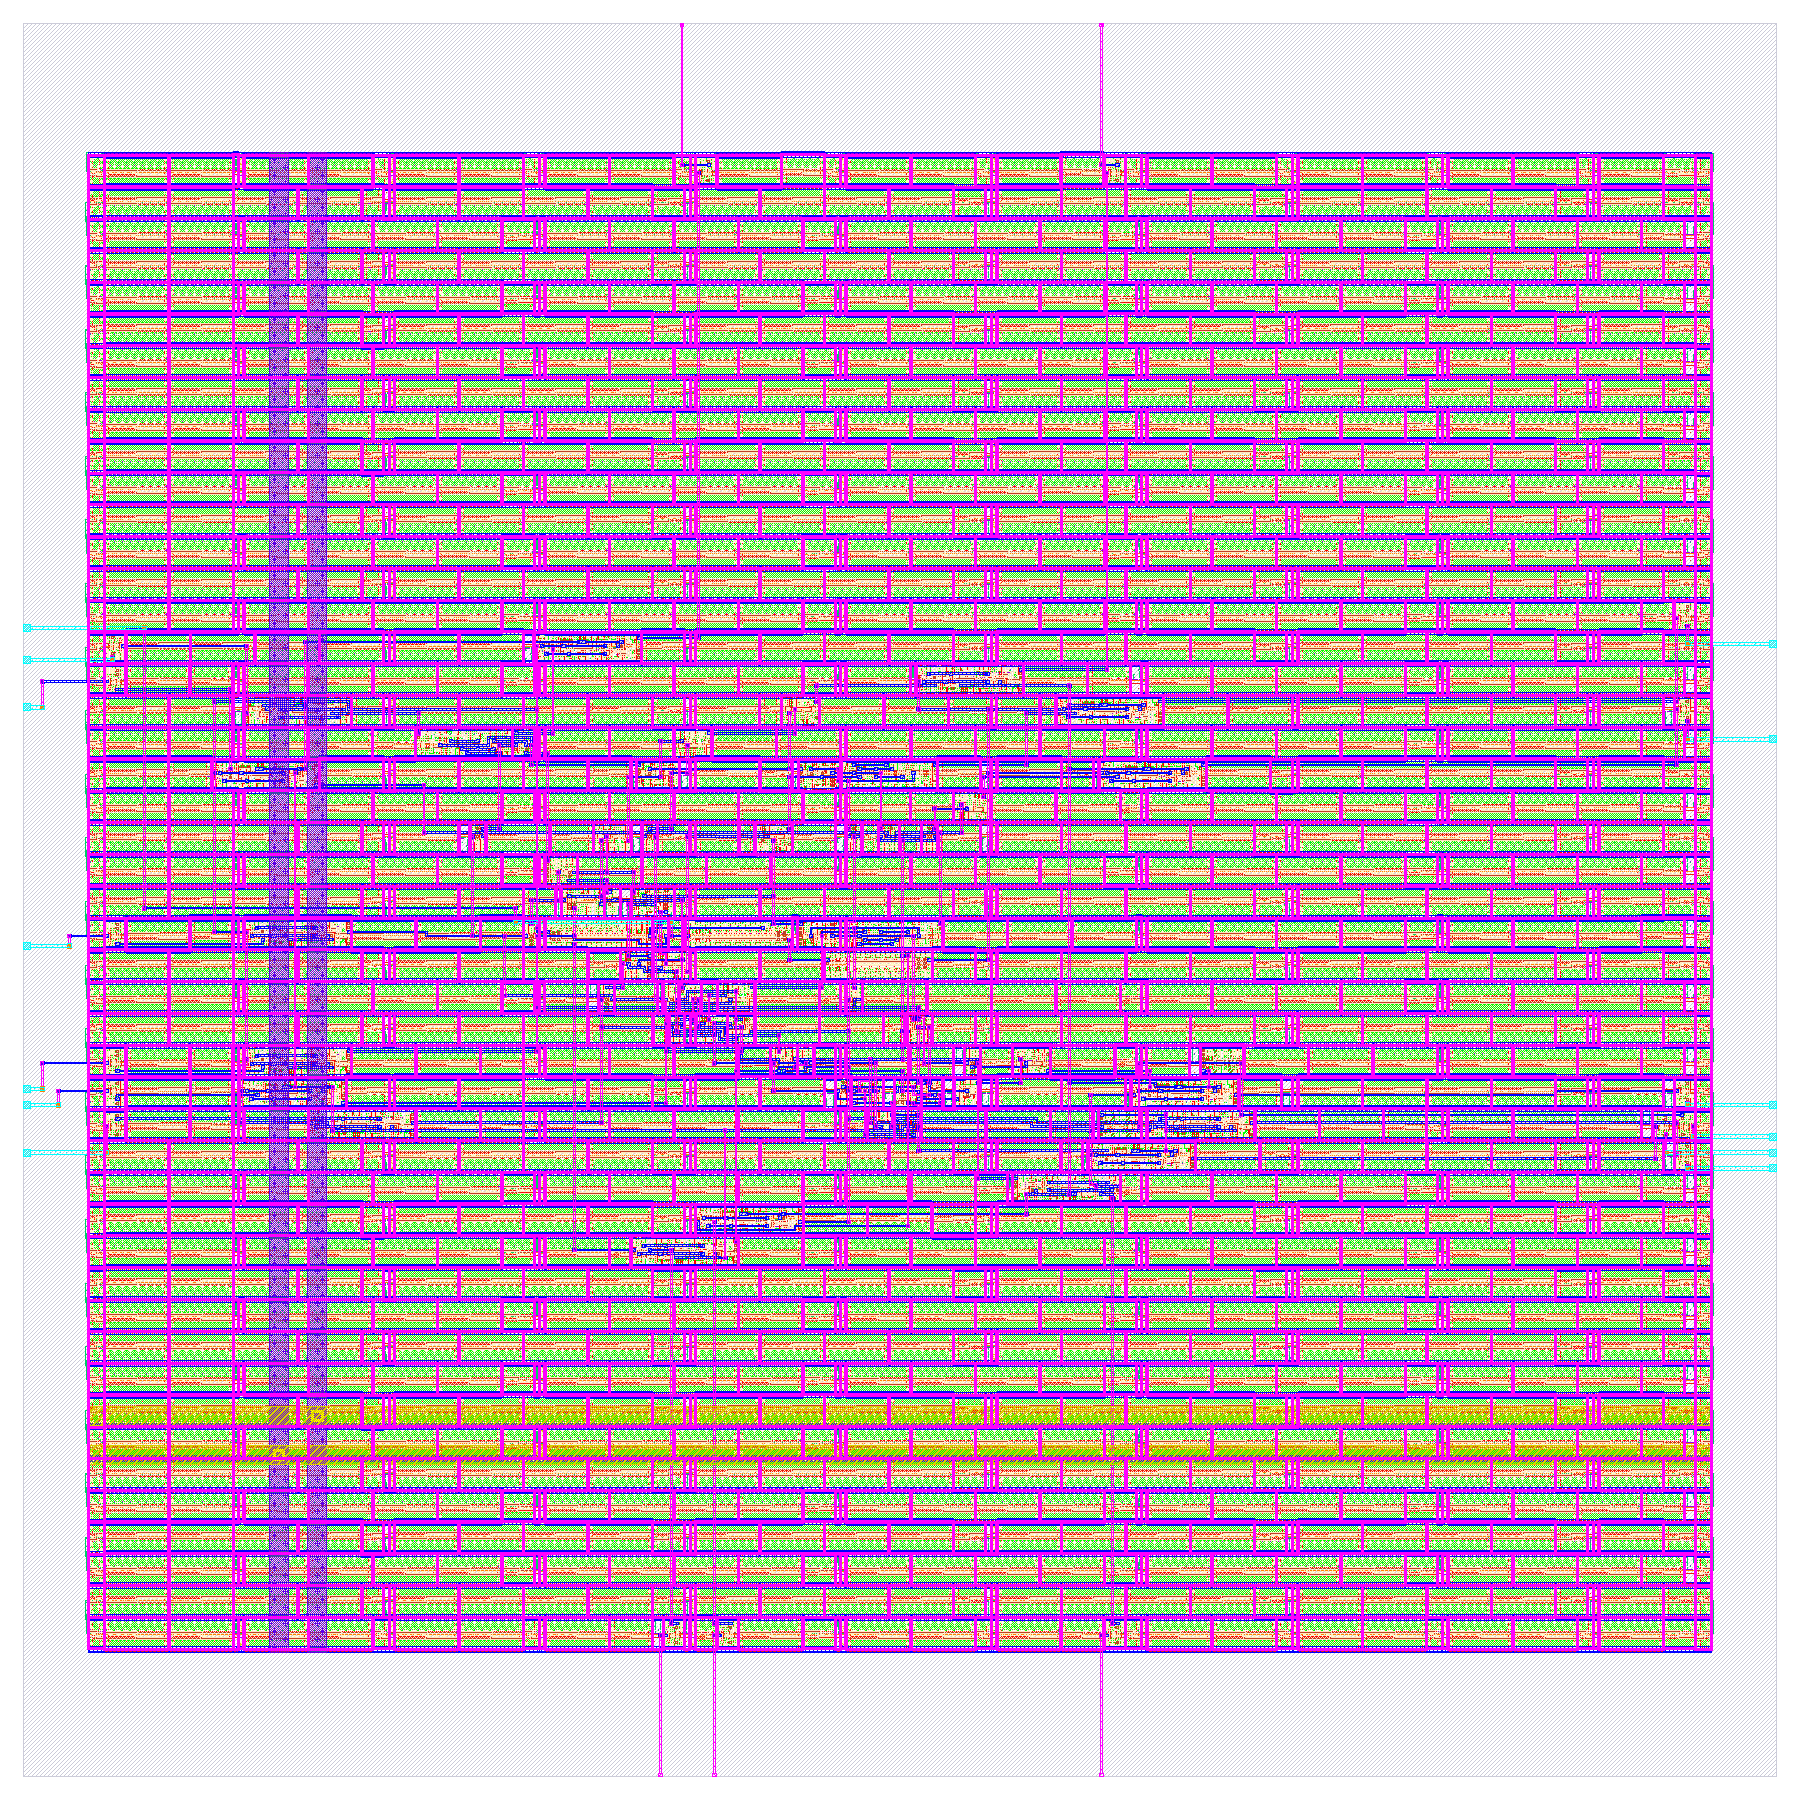
\includegraphics[width=0.78\textwidth]{figures/partD_layout_die.png}
        \caption{Whole-die view ($150\,\mu\text{m} \times 150\,\mu\text{m}$): \texttt{VPWR}/\texttt{VGND} power grid (\texttt{met4}/\texttt{met5}), perimeter I/O pins (\texttt{met2}/\texttt{met3}), 47 standard-cell rows, active logic cluster, and tap/decap/filler array.}
        \label{fig:layout_die}
    \end{subfigure}\hfill
    \begin{subfigure}[t]{0.49\textwidth}
        \centering
        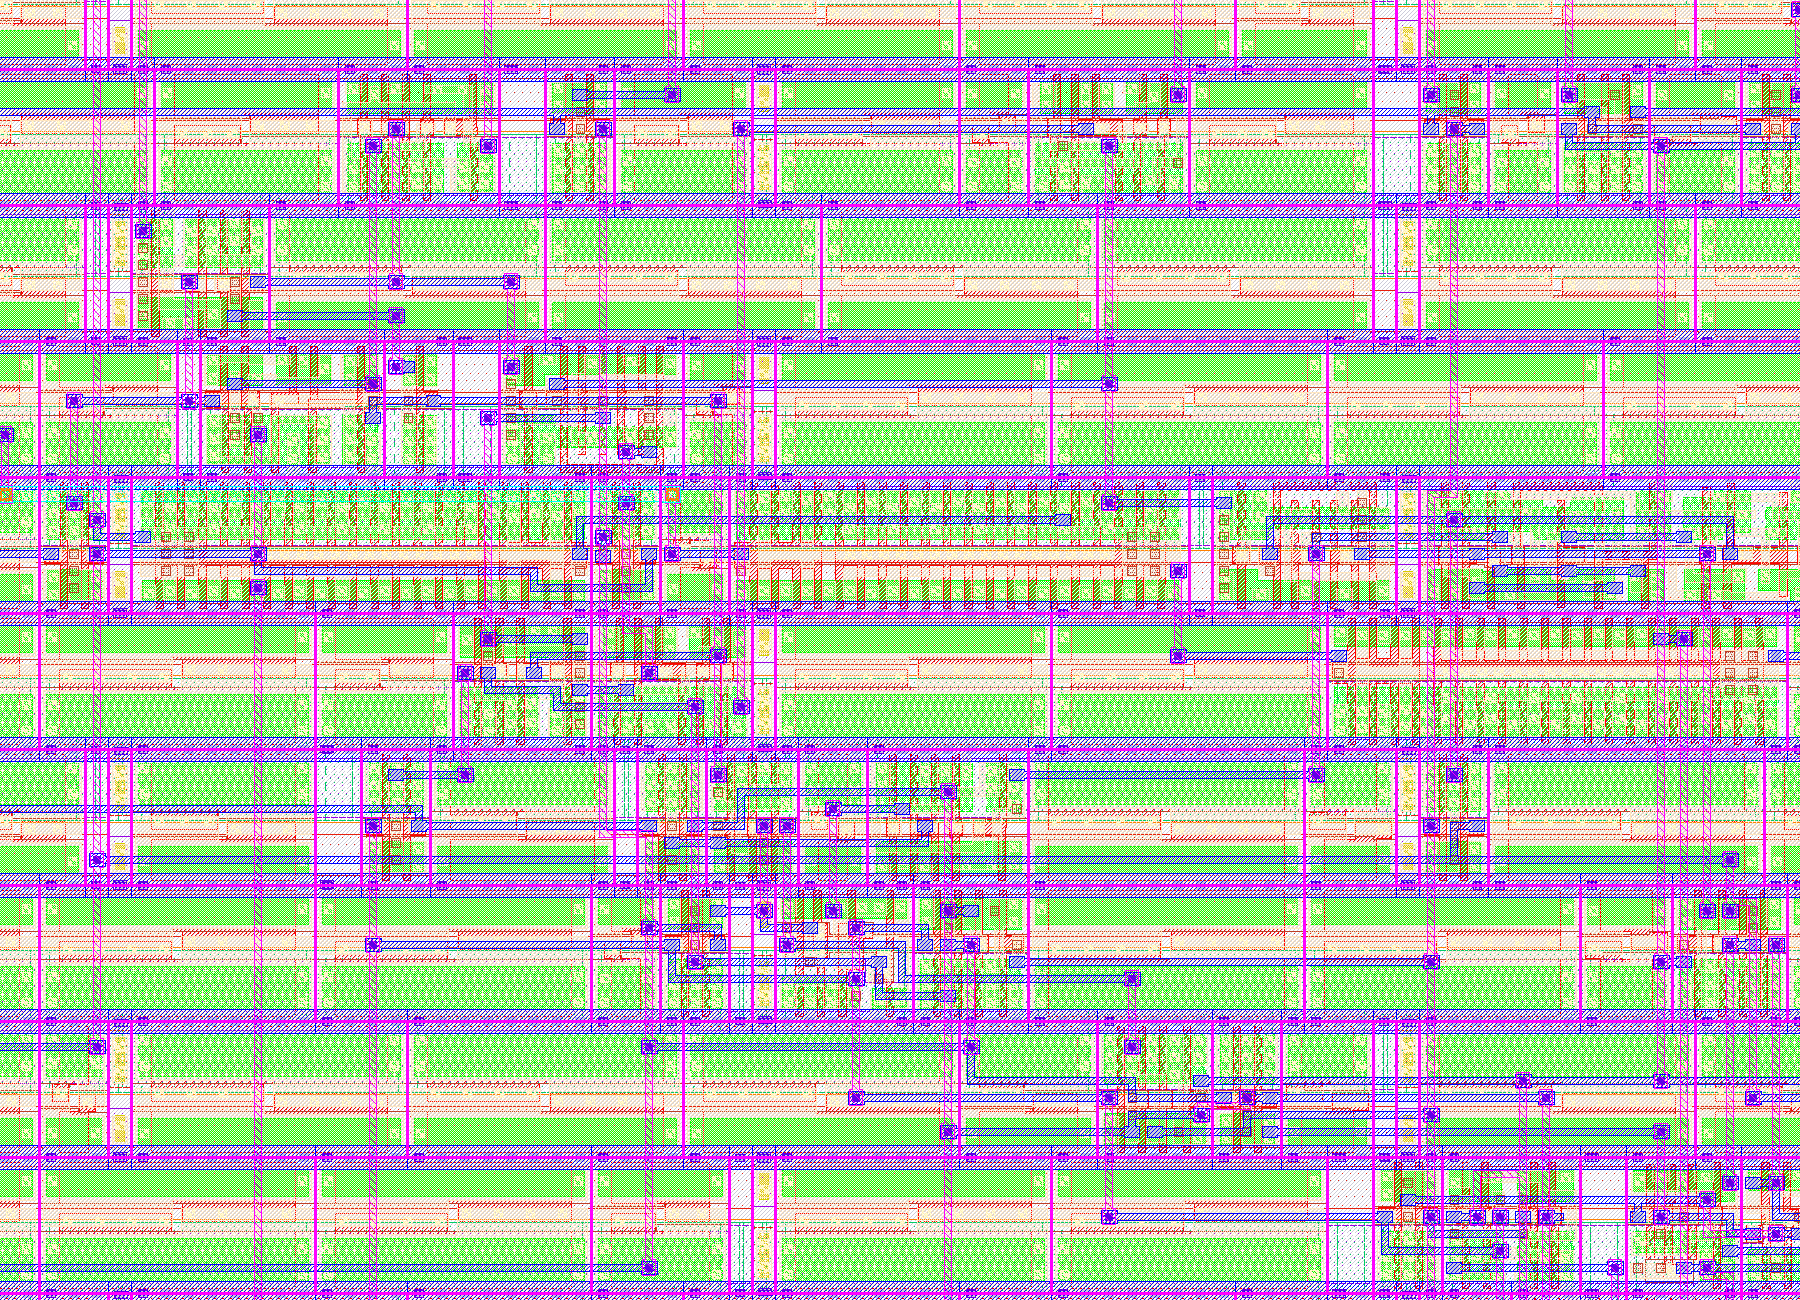
\includegraphics[width=0.88\textwidth]{figures/partD_layout_zoom.png}
        \caption{Zoomed view of standard-cell rows and metal wires: placed \texttt{dfrtp\_1}, \texttt{maj3\_1}, and \texttt{xnor2\_1} standard cells, local interconnect (\texttt{li1}), horizontal \texttt{met1}/\texttt{met3} and vertical \texttt{met2} tracks, and vias.}
        \label{fig:layout_zoom}
    \end{subfigure}
    \caption{KLayout screenshots of the final DRC- and LVS-clean layout \texttt{pnr/mult\_array.gds} (Run 8 at $T_{\text{clk}} = 7.0\text{ ns}$).}
    \label{fig:layout}
\end{figure*}

% ==================== VI. ANSWERS TO QUESTIONS ====================
\section{Answers to Questions (Section 10)}

\textbf{1) Logic Cell Count ($51$ Cells vs.\ $16 + 12 = 28$):}
Yosys produced $67 - 16 = \mathbf{51\text{ combinational logic cells}}$ ($346.582\,\mu\text{m}^2$) rather than $16 + 12 = 28$. First, each structural \texttt{full\_adder} ($\text{sum} = a \oplus b \oplus c_{\text{in}}$, $c_{\text{out}} = \text{maj}(a,b,c_{\text{in}})$) is decomposed into multiple primitive standard cells (\texttt{xnor2\_1}, \texttt{xnor3\_1}, \texttt{maj3\_1}, \texttt{nand2\_1}, AOI/OAI gates) rather than one monolithic cell. Second, the three row-LSB full adders have constant $c_{\text{in}} = 0$, which constant propagation simplifies into 2-input half-adder logic. Third, \texttt{synth -flatten} and ABC technology mapping merge and invert shared sub-expressions across the partial-product AND gates and adjacent adder stages (mapping 12 of the 16 AND gates into smaller/faster inverting \texttt{nand2\_1} and \texttt{nand4\_1} cells).

\textbf{2) Critical Path and Comparison with $2N$ Full-Adder Delays:}
From \texttt{sta/mult\_array\_timing.rpt} (Table~\ref{tab:partC_path}), the critical path starts at input register \texttt{\_106\_} (\texttt{b\_reg[0]}, \texttt{dfrtp\_1}) and ends at output register \texttt{\_100\_} (\texttt{p[6]}, \texttt{dfrtp\_1}), with a data arrival time of $2.471\text{ ns}$ and $T_{\min} = 2.604\text{ ns}$. Between these registers, the path traverses \textbf{8 combinational standard cells} (10 cells including the two flip-flops): \textbf{1 partial-product AND gate} (\texttt{\_043\_}, \texttt{and2\_0} computing $\text{pp}_0[0]$) followed by \textbf{7 addition-network cells} (\texttt{\_056\_} \texttt{or3\_1}, \texttt{\_058\_} \texttt{a32oi\_1}, \texttt{\_072\_} \texttt{o21ba\_1}, \texttt{\_073\_} \texttt{xnor2\_1}, \texttt{\_082\_} \texttt{maj3\_1}, \texttt{\_084\_} \texttt{maj3\_1}, and \texttt{\_086\_} \texttt{xnor3\_1}). This closely matches the Section 2 estimate of $\approx 2N = 8$ full-adder delays: structurally, the longest path ripples through 1 AND gate, $N-1 = 3$ vertical row transitions, and $N = 4$ horizontal stages in Row 3 ($1 + 7 = 8$ stages).

\textbf{3) Flip-Flop Area Percentage ($53.60\%$):}
The 16 \texttt{dfrtp\_1} flip-flops occupy $400.384\,\mu\text{m}^2$ out of $746.966\,\mu\text{m}^2$, or \textbf{53.60\%} of the total cell area ($25.024\,\mu\text{m}^2$ per DFF vs.\ $346.582\,\mu\text{m}^2$ for all 51 combinational cells). Each master-slave edge-triggered D flip-flop with asynchronous reset contains two clocked latches, transmission gates, internal clock buffers, and reset transistors ($\sim 24\text{--}28$ transistors, $6.67\times$ the area of a $3.754\,\mu\text{m}^2$ \texttt{nand2\_1} gate). Moreover, register count scales linearly as $4N$ ($2N$ input $+ 2N$ output FFs) while the combinational array scales quadratically as $\mathcal{O}(N^2)$ ($N^2$ AND gates $+ N(N-1)$ adders); at $N = 4$, $4N = 16$ equals $N^2 = 16$, making flip-flop area dominant.

\textbf{4) Post-Route $F_{\max}$ vs.\ Part C $F_{\max}$ and Added Physical Cells:}
Post-route $F_{\max}$ is \textbf{153.01\,MHz} in the worst-case signoff corner (\texttt{max\_ss\_100C\_1v60}, setup slack $+0.465\text{ ns}$ at $7.0\text{ ns}$) and \textbf{316.34\,MHz} in the nominal corner (\texttt{nom\_tt\_025C\_1v80}, setup slack $+3.839\text{ ns}$), compared to \textbf{384.02\,MHz} in Part C. In the same nominal corner, $F_{\max}$ drops by $17.6\%$ due to extracted RC parasitics across $2,328\,\mu\text{m}$ of metal wiring and $530$ vias, clock-tree skew ($0.265\text{ ns}$), and buffer insertion; multi-corner signoff is further limited by the slow-slow corner ($1.60\text{ V}, 100\,^\circ\text{C}$, $60.2\%$ lower $F_{\max}$) where low supply voltage and high temperature reduce transistor drive current. While OpenROAD remapped the 51 combinational cells into 45 cells (keeping 16 DFFs), the flow increased total cell count from 67 to \textbf{1,883 cells} by adding: (1) \textbf{3 clock buffers} (\texttt{clkbuf\_*}) during CTS to balance clock arrival across all 16 flip-flops; (2) \textbf{19 timing/slew repair buffers} (\texttt{buf\_*}, \texttt{clkbuf\_*}, \texttt{dlygate*}) to buffer I/O nets and fix max-slew/hold constraints; (3) \textbf{245 well/substrate tap cells} (\texttt{tapvpwrvgnd\_1}) to bias the p-substrate to \texttt{VGND} and n-well to \texttt{VPWR} against CMOS latch-up; and (4) \textbf{1,555 filler and decoupling capacitor cells} (\texttt{fill\_*}, \texttt{decap\_*}) to maintain continuous n-well/power rails for DRC compliance and suppress dynamic IR drop.

\textbf{5) DRC and LVS Verification and Manufacturing Signoff:}
\textbf{Design Rule Checking (DRC)} (Magic and KLayout: \textbf{0 errors}) verifies that all mask polygons obey the SkyWater 130\,nm geometric and process rules (minimum metal width, spacing, via enclosure, well overlap, and antenna rules). \textbf{Layout Versus Schematic (LVS)} (Netgen: \textbf{0 errors}) extracts the physical transistor/cell netlist from the layout and compares it against the synthesized netlist (\texttt{synth/mult\_array\_netlist.v}) to confirm identical devices, nets, and pins. Both must pass before fabrication because DRC violations cause physical manufacturing defects (shorts, opens, oxide breakdown), whereas LVS violations mean a physically manufacturable chip implements the wrong circuit connectivity.

\textbf{6) Scaling from a 4-Bit to an 8-Bit Array Multiplier:}
Using the Section 2 formulas ($\text{FA}(N) = N(N-1)$ full adders, $N^2$ AND gates, and critical path $\approx 2N$ full-adder delays):
\begin{itemize}
    \item \textbf{Full Adders}: At $N = 4$, $\text{FA}_4 = 4(3) = 12$ full adders ($16$ AND gates). At $N = 8$, $\text{FA}_8 = 8(7) = \mathbf{56\text{ full adders}}$ ($64$ AND gates), an increase of $56 - 12 = \mathbf{+44\text{ full adders}}$ or $\frac{56}{12} = \mathbf{4.67\times}$ (quadratic $\mathcal{O}(N^2)$ growth).
    \item \textbf{Critical Path Delay}: Using $\approx 2N$ full-adder delays, the critical path grows from $2(4) = 8$ to $2(8) = \mathbf{16\text{ full-adder delays}}$ (\textbf{$2.0\times$ increase}, linear $\mathcal{O}(N)$ growth). Scaling from our Part C pre-layout measurement ($T_{\min,4} = 2.604\text{ ns}$, with $2.083\text{ ns}$ combinational delay across 1 AND $+ 7$ adder stages $\approx 0.272\text{ ns}$/FA), doubling the path gives $T_{\min,8} \approx 2 \times 2.604 = \mathbf{5.21\text{ ns}}$ ($F_{\max,8} \approx \mathbf{192\text{ MHz}}$), or using $(2N-1) = 15$ full-adder stages plus 1 AND gate and flip-flop overhead: $T_{\min,8} \approx 0.388 + 0.180 + 15(0.272) - 0.134 = \mathbf{4.51\text{ ns}}$ ($F_{\max,8} \approx \mathbf{221.6\text{ MHz}}$).
\end{itemize}

% ==================== VII. CONCLUSION ====================
\section{Conclusion}
A 4-bit unsigned registered array multiplier (\texttt{mult\_array}) was designed structurally in Verilog using 16 AND gates, 12 full adders, and 16 flip-flops, verified across all 256 vectors in RTL and gate-level simulation (\texttt{PASS: 256 vectors checked, 0 errors}) alongside a 95-error fault-injection test, synthesized with Yosys to 67 \texttt{sky130\_fd\_sc\_hd} cells ($746.966\,\mu\text{m}^2$, $53.60\%$ sequential area), analyzed in OpenSTA ($T_{\min} = 2.604\text{ ns}$, $F_{\max} = 384.02\text{ MHz}$), and implemented through 8 LibreLane/OpenROAD runs into a DRC- and LVS-clean $150\,\mu\text{m} \times 150\,\mu\text{m}$ GDSII layout achieving $153.01\text{ MHz}$ multi-corner signoff operation ($316.34\text{ MHz}$ nominal).

% ==================== APPENDIX ====================
\section*{Appendix}
\subsection*{A. Complete Simulation Logs (Passed Run, GLS, and 95-Error Injection)}
\label{app:logs}

\begin{lstlisting}[title={\textbf{1. Part A Behavioral RTL Pass Log \& Part B GLS Pass Log}}]
# Part A Behavioral RTL Simulation (vvp sim)
VCD info: dumpfile mult.vcd opened for output.
PASS: 256 vectors checked, 0 errors
tb/tb_mult.v:75: $finish called at 5146000 (1ps)

# Part B Gate-Level Simulation (vvp gls)
VCD info: dumpfile mult.vcd opened for output.
PASS: 256 vectors checked, 0 errors
tb/tb_mult.v:77: $finish called at 5147000 (1ps)
\end{lstlisting}

\begin{lstlisting}[title={\textbf{2. Part A Task 6 Error-Injection Log (\texttt{sum = a \^{} b} --- All 95 Mismatches)}},basicstyle=\ttfamily\tiny]
VCD info: dumpfile mult.vcd opened for output.
a=3  b=3  exp=9   got=5   | a=11 b=6  exp=66  got=122
a=3  b=6  exp=18  got=10  | a=11 b=7  exp=77  got=81
a=3  b=7  exp=21  got=9   | a=11 b=9  exp=99  got=83
a=3  b=11 exp=33  got=29  | a=11 b=10 exp=110 got=78
a=3  b=12 exp=36  got=20  | a=11 b=11 exp=121 got=229
a=3  b=13 exp=39  got=23  | a=11 b=12 exp=132 got=244
a=3  b=14 exp=42  got=18  | a=11 b=13 exp=143 got=127
a=3  b=15 exp=45  got=17  | a=11 b=14 exp=154 got=162
a=5  b=5  exp=25  got=17  | a=11 b=15 exp=165 got=137
a=5  b=7  exp=35  got=27  | a=12 b=3  exp=36  got=52
a=5  b=10 exp=50  got=34  | a=12 b=6  exp=72  got=104
a=5  b=11 exp=55  got=39  | a=12 b=7  exp=84  got=68
a=5  b=13 exp=65  got=57  | a=12 b=11 exp=132 got=212
a=5  b=14 exp=70  got=54  | a=12 b=12 exp=144 got=208
a=5  b=15 exp=75  got=51  | a=12 b=13 exp=156 got=220
a=6  b=3  exp=18  got=10  | a=12 b=14 exp=168 got=136
a=6  b=6  exp=36  got=20  | a=12 b=15 exp=180 got=164
a=6  b=7  exp=42  got=18  | a=13 b=3  exp=39  got=55
a=6  b=11 exp=66  got=58  | a=13 b=5  exp=65  got=121
a=6  b=12 exp=72  got=40  | a=13 b=6  exp=78  got=110
a=6  b=13 exp=78  got=46  | a=13 b=7  exp=91  got=67
a=6  b=14 exp=84  got=36  | a=13 b=9  exp=117 got=101
a=6  b=15 exp=90  got=34  | a=13 b=10 exp=130 got=242
a=7  b=3  exp=21  got=9   | a=13 b=11 exp=143 got=223
a=7  b=5  exp=35  got=27  | a=13 b=12 exp=156 got=220
a=7  b=6  exp=42  got=18  | a=13 b=13 exp=169 got=145
a=7  b=7  exp=49  got=21  | a=13 b=14 exp=182 got=134
a=7  b=10 exp=70  got=54  | a=13 b=15 exp=195 got=171
a=7  b=11 exp=77  got=49  | a=14 b=3  exp=42  got=50
a=7  b=12 exp=84  got=36  | a=14 b=5  exp=70  got=118
a=7  b=13 exp=91  got=35  | a=14 b=6  exp=84  got=100
a=7  b=14 exp=98  got=42  | a=14 b=7  exp=98  got=74
a=7  b=15 exp=105 got=45  | a=14 b=10 exp=140 got=236
a=9  b=9  exp=81  got=65  | a=14 b=11 exp=154 got=194
a=9  b=11 exp=99  got=83  | a=14 b=12 exp=168 got=200
a=9  b=13 exp=117 got=101 | a=14 b=13 exp=182 got=134
a=9  b=15 exp=135 got=247 | a=14 b=14 exp=196 got=148
a=10 b=5  exp=50  got=34  | a=14 b=15 exp=210 got=186
a=10 b=7  exp=70  got=118 | a=15 b=3  exp=45  got=49
a=10 b=10 exp=100 got=68  | a=15 b=5  exp=75  got=115
a=10 b=11 exp=110 got=78  | a=15 b=6  exp=90  got=98
a=10 b=13 exp=130 got=114 | a=15 b=7  exp=105 got=77
a=10 b=14 exp=140 got=236 | a=15 b=9  exp=135 got=247
a=10 b=15 exp=150 got=166 | a=15 b=10 exp=150 got=230
a=11 b=3  exp=33  got=61  | a=15 b=11 exp=165 got=201
a=11 b=5  exp=55  got=39  | a=15 b=12 exp=180 got=196
a=15 b=13 exp=195 got=139 | a=15 b=14 exp=210 got=154
a=15 b=15 exp=225 got=181 |
FAIL: 256 vectors checked, 95 errors
tb/tb_mult.v:75: $finish called at 5146000 (1ps)
\end{lstlisting}

\subsection*{B. OpenSTA Critical Path Timing Report (\texttt{sta/mult\_array\_timing.rpt})}
\begin{lstlisting}[title={\textbf{OpenSTA Critical Path Report ($T_{\text{clk}} = 2.60\text{ ns}$ and $10.00\text{ ns}$)}},basicstyle=\ttfamily\tiny]
Startpoint: rst_n (input port clocked by clk) -> Endpoint: _094_ (recovery)
Path Group: asynchronous | Path Type: max | Arrival: 1.000 ns
Required: 2.828 ns (at 2.60 ns) -> Slack: +1.828 ns (MET) [+9.228 ns at 10.0 ns]

Startpoint: _106_ (rising edge-triggered flip-flop clocked by clk, b_reg[0])
Endpoint:   _100_ (rising edge-triggered flip-flop clocked by clk, p[6])
Path Group: clk   | Path Type: max
   Delay     Time   Description
-----------------------------------------------------------
   0.000    0.000 ^ _106_/CLK (sky130_fd_sc_hd__dfrtp_1)
   0.388    0.388 v _106_/Q   (sky130_fd_sc_hd__dfrtp_1)
   0.180    0.568 v _043_/X   (sky130_fd_sc_hd__and2_0)
   0.391    0.959 v _056_/X   (sky130_fd_sc_hd__or3_1)
   0.250    1.208 ^ _058_/Y   (sky130_fd_sc_hd__a32oi_1)
   0.198    1.406 v _072_/X   (sky130_fd_sc_hd__o21ba_1)
   0.147    1.553 v _073_/Y   (sky130_fd_sc_hd__xnor2_1)
   0.385    1.937 v _082_/X   (sky130_fd_sc_hd__maj3_1)
   0.358    2.295 v _084_/X   (sky130_fd_sc_hd__maj3_1)
   0.175    2.471 v _086_/X   (sky130_fd_sc_hd__xnor3_1)
   0.000    2.471 v _100_/D   (sky130_fd_sc_hd__dfrtp_1)
            2.471   data arrival time
   2.600    2.600 ^ _100_/CLK (clock clk rise edge; 10.000 ns at T=10.0 ns)
  -0.134    2.466   library setup time (9.866 ns required at T=10.0 ns)
-----------------------------------------------------------
           -0.004   slack at T = 2.60 ns (+7.396 ns slack MET at T = 10.00 ns)
\end{lstlisting}

% ==================== VIII. TEAM CONTRIBUTIONS ====================
\section{Team Contributions}

\begin{table}[!h]
    \centering
    \caption{Alternating Part-Wise Team Contribution Breakdown.}
    \label{tab:contributions}
    \footnotesize
    \setlength{\tabcolsep}{4pt}
    \begin{tabularx}{\columnwidth}{@{}l l >{\raggedright\arraybackslash}X r@{}}
        \toprule
        \textbf{Part} & \textbf{Team Member} & \textbf{Deliverables \& Report Scope} & \textbf{Weight} \\
        \midrule
        \textbf{Part A} & Manikya Pant (\texttt{2023112024}) & RTL design (\texttt{full\_adder.v}, \texttt{mult\_array.v}), testbench (\texttt{tb\_mult.v}), 256-vector \& fault sims, waveform, hand trace, block diagram, Q1 & 30\% \\
        \midrule
        \textbf{Part B} & Aryan Agrawal (\texttt{2023102050}) & Yosys synthesis (\texttt{synth.tcl}, \texttt{mult\_array\_netlist.v}), cell/area analysis (\texttt{mult\_array\_stat.rpt}), gate-level simulation, Q3 & 20\% \\
        \midrule
        \textbf{Part C} & Manikya Pant (\texttt{2023112024}) & OpenSTA script (\texttt{sta.tcl}), $T_{\min}$/$F_{\max}$ timing analysis, 8-cell critical path trace (\texttt{mult\_array\_timing.rpt}), Q2, Q6 & 20\% \\
        \midrule
        \textbf{Part D} & Aryan Agrawal (\texttt{2023102050}) & LibreLane PnR (\texttt{config.json}), 8-run \texttt{CLOCK\_PERIOD} sweep, \texttt{metrics.json}, KLayout GDS screenshots (\texttt{mult\_array.gds}), Q4, Q5 & 30\% \\
        \midrule
        \multicolumn{2}{@{}l}{\textbf{Manikya Pant (\texttt{2023112024})}} & \textbf{Part A (30\%) + Part C (20\%)} & \textbf{50\%} \\
        \multicolumn{2}{@{}l}{\textbf{Aryan Agrawal (\texttt{2023102050})}} & \textbf{Part B (20\%) + Part D (30\%)} & \textbf{50\%} \\
        \bottomrule
    \end{tabularx}
\end{table}

\end{document}
